% created by hand
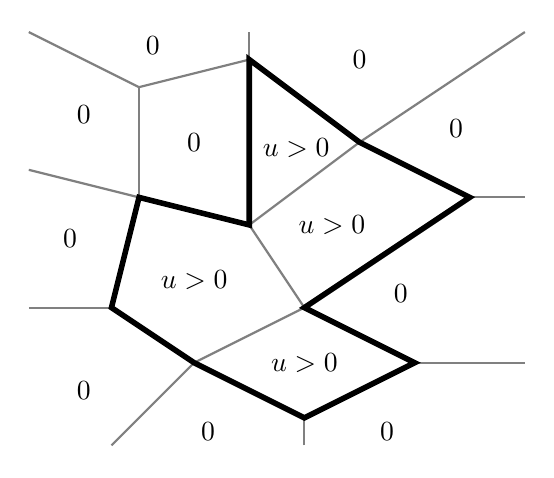
\begin{tikzpicture}[scale=0.35]
  \draw[gray, thick] (3,0) -- (6,3);
  \draw[gray, thick] (0,5) -- (3,5);
  \draw[gray, thick] (0,10) -- (4,9);
  \draw[gray, thick] (0,15) -- (4,13);
  \draw[gray, thick] (4,13) -- (4,9);
  \draw[gray, thick] (4,13) -- (8,14);
  \draw[gray, thick] (8,14) -- (8,15);
  \draw[gray, thick] (12,11) -- (18,15);
  \draw[gray, thick] (10,5) -- (14,3);
  \draw[gray, thick] (10,1) -- (14,3);
  \draw[gray, thick] (14,3) -- (18,3);
  \draw[gray, thick] (6,3) -- (10,1);
  \draw[gray, thick] (6,3) -- (10,5);
  \draw[gray, thick] (10,0) -- (10,1);
  \draw[gray, thick] (10,5) -- (8,8);
  \draw[gray, thick] (8,8) -- (12,11);
  \draw[gray, thick] (16,9) -- (18,9);

  % the free boundary is bold
  \draw[line width=2.0pt] (6,3) -- (3,5) -- (4,9) -- (8,8) -- (8,14) --
                          (12,11) -- (16,9) -- (10,5) -- (14,3) -- (10,1) -- cycle;
  % label cells with positive thickness
  \draw (6,6) node {$u>0$};
  \draw (11,8) node {$u>0$};
  \draw (9.7,10.8) node {$u>0$};
  \draw (10,3) node {$u>0$};
  % label cells with zero thickness
  \draw (2,2) node {$0$};
  \draw (1.5,7.5) node {$0$};
  \draw (2,12) node {$0$};
  \draw (4.5,14.5) node {$0$};
  \draw (6,11) node {$0$};
  \draw (12,14) node {$0$};
  \draw (15.5,11.5) node {$0$};
  \draw (13.5,5.5) node {$0$};
  \draw (13,0.5) node {$0$};
  \draw (6.5,0.5) node {$0$};
\end{tikzpicture}
